
\documentclass{article}
\usepackage{amsmath}
\usepackage[utf8]{inputenc}
\usepackage{ctex}
\usepackage{indentfirst}

\usepackage{graphicx}

\usepackage{listings}
\usepackage{color}

\lstset{
    language=Python, % 设置语言
    basicstyle=\ttfamily, % 基本字体样式
    keywordstyle=\color{blue}, % 关键词的颜色
    commentstyle=\color{green}, % 注释的颜色
    stringstyle=\color{red}, % 字符串的颜色
    showstringspaces=false, % 不显示字符串间隙
    numbers=left, % 显示行号
    numberstyle=\tiny\color{gray}, % 行号样式
    breaklines=true, % 自动换行
    frame=single % 给代码框加一个边框
}


\setlength{\parindent}{2em}

\begin{document}

\begin{center}
    \Large \textbf{Lab1 实验报告}\\
    \vspace{1em}
    姓名:~~学号:~~班级:
\end{center}

\section{实验概览}
    本次实验主要学习了图像在计算机中的存储形式和OpenCV库相关函数的使用。

    对于一张图片,其基本元素为像素。常见的图像类型有灰度图和彩色图两种。
    对于灰度图,图像由一个\( W \times H \) 的灰度值矩阵组成。
    \( W \) 为构成宽度的像素数目,\( H \) 为构成高度的像素数目。
    灰度值的取值范围为 \([0, 255]\),数值越高意味着颜色越淡。
    其中,0 代表黑色,255 代表白色。

    而对于彩色图像而言,图像由一个 \( W \times H \times 3 \) 的高维矩阵构成,
    分别由红色 (R)、绿色 (G)、蓝色 (B) 三维描述对应颜色的分量。
    特别地,对于彩色图像与灰度图像的转化,我们有一个常用公式:

\[
\text{Gray} = 0.299R + 0.587G + 0.114B
\]

    对于计算机而言,图片本身直接蕴含的信息不多,需要对其做特征提取。本次实验主要以图像直方图特征来反映图片的特征。

    图像的直方图特征是一种全局统计特征,描述了图像的某一数值特性的分布情况,反映了图像的大体风格。
    在本次实验中,主要实现了颜色直方图,灰度直方图和梯度直方图三种特征图像的提取,
    分别反映了图像全局的主体色调,灰度图像的明暗程度,图像纹理的疏密程度。

    OpenCV (Open Source Computer Vision Library)是一个开源的计算机视觉和机器学习软件库。
    它提供了丰富的工具,用于图像处理、视频分析、物体识别、深度学习等。
    广泛应用于实时应用,如人脸识别、自主驾驶和增强现实。
    本次实验主要使用其python接口实现图像读入等功能。
    
\section{练习题的解决思路}
    主要根据图像的定义实现,

    对于练习题1,彩色图像I(x, y, c)的颜色直方图是它三个颜色分量总能量的相对比例。
    通过遍历每一个点,将对应颜色分量累加得到R,G,B三个数,再分别除以三者之和得到对应的比例。公式如下:

    \[E(c) = \sum_{x = 0}^{W - 1} \sum_{y = 0}^{H - 1}I(x, y, c) \]
    \[H(c) = \frac{E(c)}{\sum\limits_{i\in {R,G,B}}^{} E(i)}\]

    而后通过matplotlib库中的pyplot函数实现绘图。\\

    对于练习题2,灰度直方图同理彩色图像的颜色直方图,遍历采样并累加得到结果。
    灰度图像 \( I(x, y) \) 的灰度直方图定义为各灰度值像素数目的相对比例。
    考虑到样本点数固定为\( W \times H \), 每次计数时加\(\frac{1}{ W \times H} \)即可。公式如下:

    图像中灰度值为 \( i \) 的像素总个数为:
    \[
    N(i) = \sum_{x=0}^{W-1} \sum_{y=0}^{H-1} \left( I(x, y) == i ? 1 : 0 \right)
    \]

    灰度直方图:
    \[
    H(i) = \frac{N(i)}{\sum\limits_{j=0}^{255} N(j)}, \quad i = 0, \dots, 255
    \]


    而梯度直方图略有不同。假设 \( I(x, y) \) 表示一幅灰度图像,则

    X 方向的梯度定义为:
    \[
    I_x(x, y) = \frac{\partial I(x, y)}{\partial x} = I(x+1, y) - I(x, y)
    \]

    Y 方向的梯度定义为:
    \[
    I_y(x, y) = \frac{\partial I(x, y)}{\partial y} = I(x, y+1) - I(x, y)
    \]

    梯度强度定义为
    \[
    M(x, y) = \sqrt{I_x(x, y)^2 + I_y(x, y)^2}
    \]

    由此,忽略边缘点的情况下,我们可以统计\((1 ~\textasciitilde ~(W - 2))
    \times (1 ~\textasciitilde ~(H - 2))\)范围内的梯度情况。
    将对应梯度强度取整后,可得到梯度强度分布的情况。公式如下:

    图像中梯度强度值为 \( i \) 的像素总个数为:
    \[
    N(i) = \sum_{x=1}^{W-2} \sum_{y=1}^{H-2} \left( floor(M(x, y)) == i ? 1 : 0 \right)
    \]

    灰度直方图:
    \[
    H(i) = \frac{N(i)}{\sum\limits_{j=0}^{360} N(j)}, \quad i = 0, \dots, 360
    \]

\section{代码运行结果}


\begin{figure}[h]
    \centering
    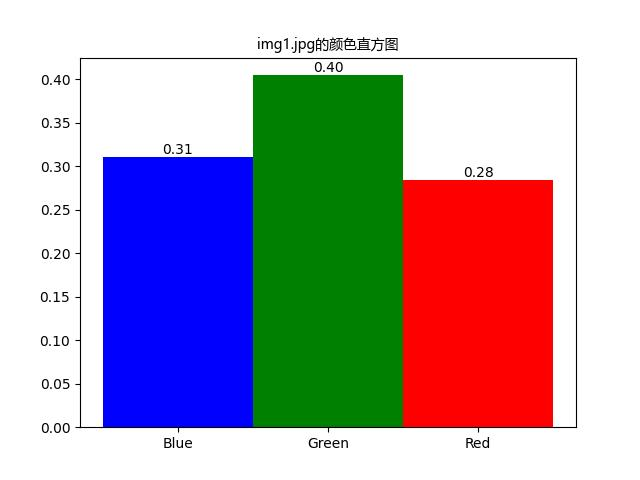
\includegraphics[width=0.3\textwidth]{./colormap/img1}
    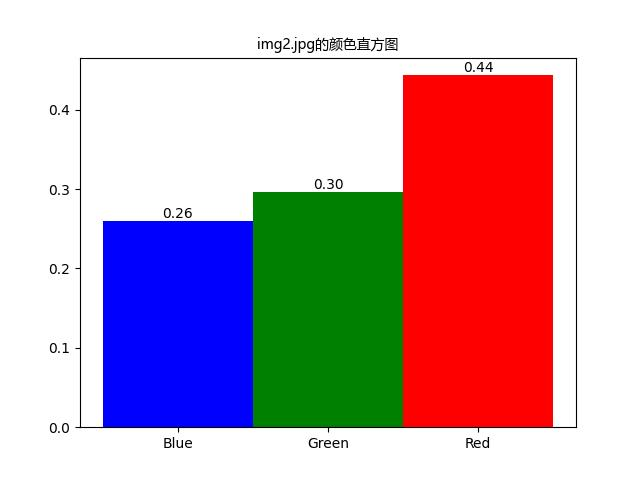
\includegraphics[width=0.3\textwidth]{./colormap/img2}
    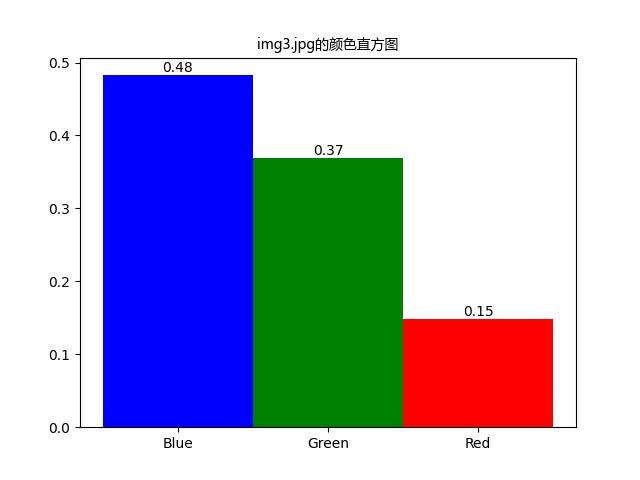
\includegraphics[width=0.3\textwidth]{./colormap/img3}
    \caption{颜色直方图}
\end{figure}

\begin{figure}[h]
    \centering
    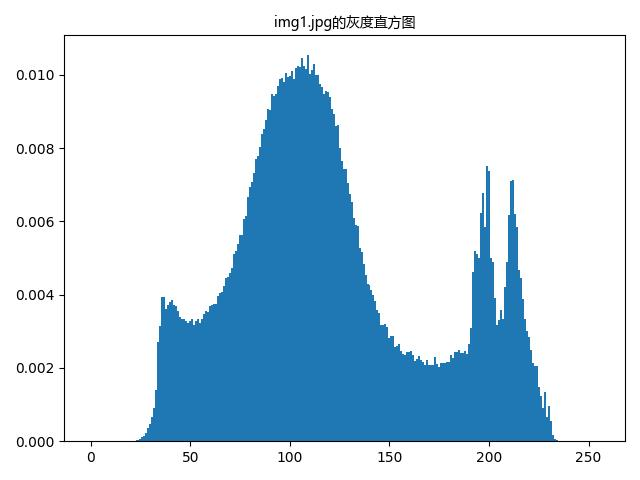
\includegraphics[width=0.3\textwidth]{./greymap/img1}
    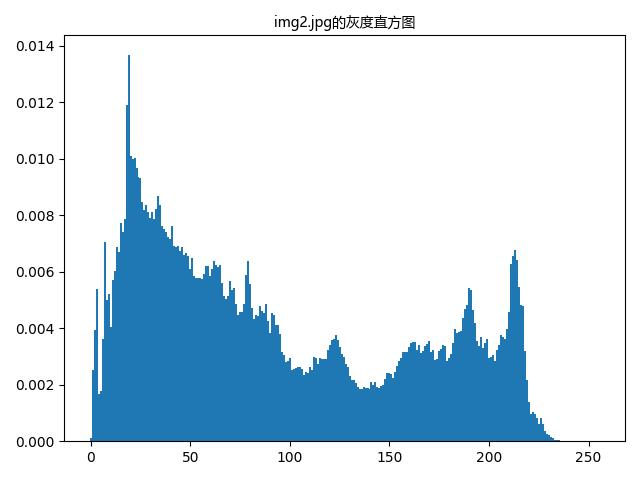
\includegraphics[width=0.3\textwidth]{./greymap/img2}
    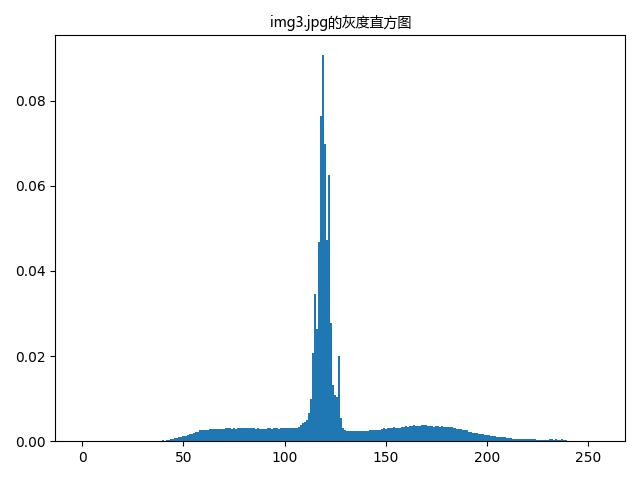
\includegraphics[width=0.3\textwidth]{./greymap/img3}
    \caption{灰度直方图}
\end{figure}

\begin{figure}[h]
    \centering
    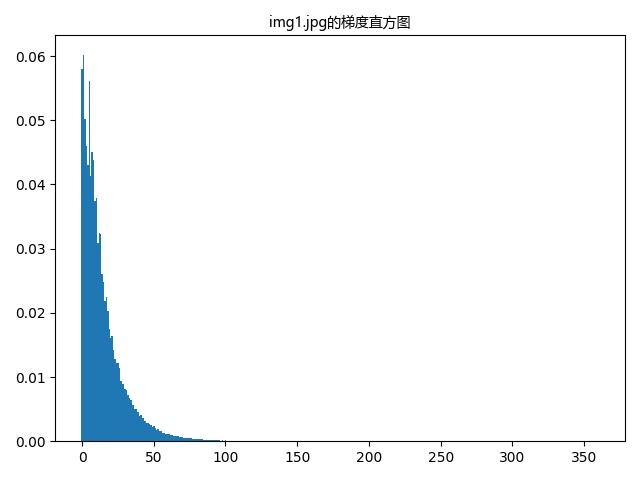
\includegraphics[width=0.3\textwidth]{./gradmap/img1}
    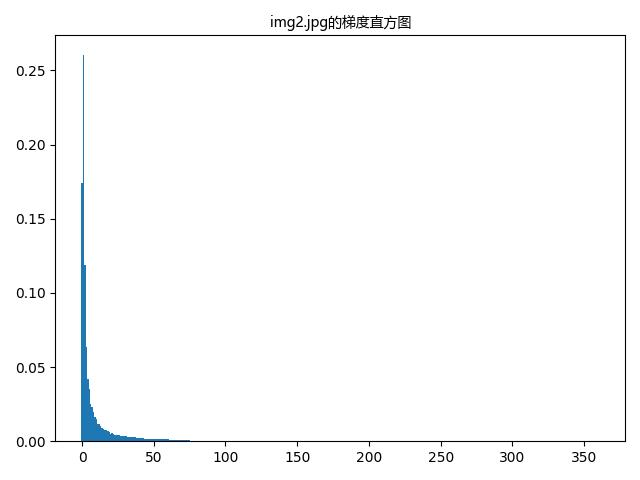
\includegraphics[width=0.3\textwidth]{./gradmap/img2}
    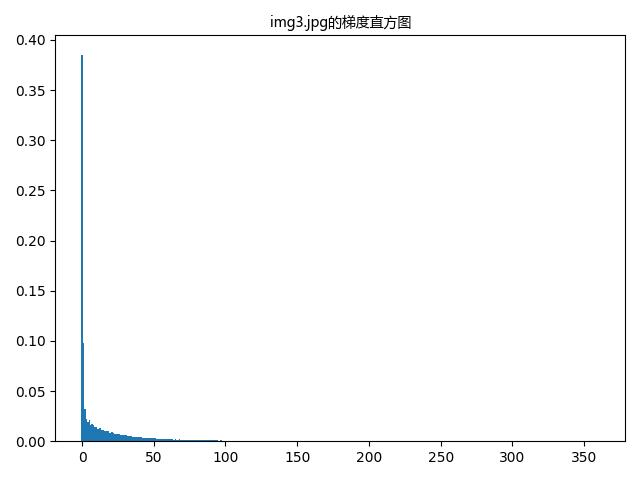
\includegraphics[width=0.3\textwidth]{./gradmap/img3}
    \caption{梯度直方图}
\end{figure}

\section{实验结果分析与思考}
\subsection{拓展思考回答}
    Q1: 示例代码中的
\begin{lstlisting}
cv2.cvtColor(img_bgr,cv2.COLOR_BGR2RGB)
\end{lstlisting}
    的作用是什么?

    A: OpenCV读取的图像默认是BGR顺序而不是RGB,由BGR2RGB可以推断出这里改变了颜色的存储顺序,
    使之更符合我们的阅读和使用习惯。

    Q2: 如何使得pyplot正确显示灰度图的颜色?

    A: 默认情况下,imshow使用伪彩色,以帮助区分不同的数值。所以对于灰度图片需要指定其显示格式。
    具体而言,可以使用以下命令

    \begin{lstlisting}
plt.imshow(image, cmap='gray', vmin=0, vmax=255)
    \end{lstlisting}
来指定输出灰度图及其灰度范围
    
\subsection{实验结果分析}

\begin{figure}[h]
    \centering
    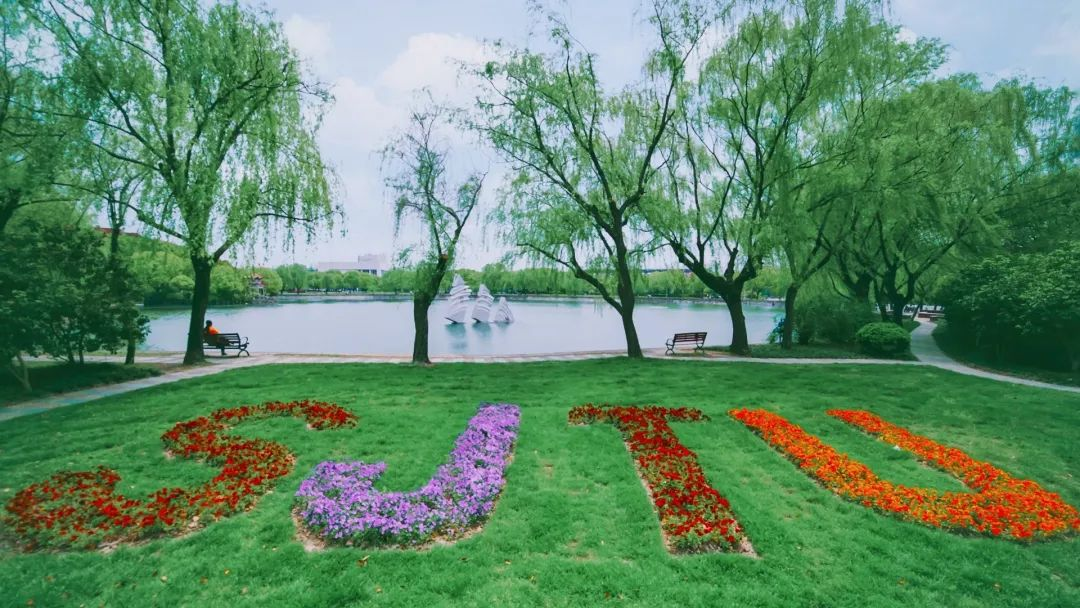
\includegraphics[width=0.3\textwidth]{./images/img1}
    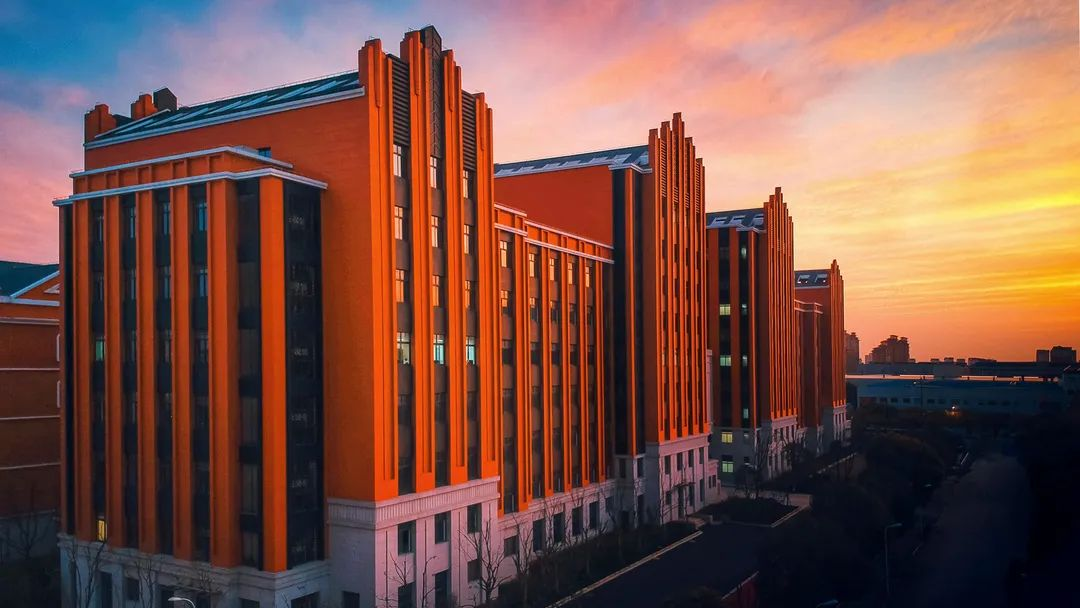
\includegraphics[width=0.3\textwidth]{./images/img2}
    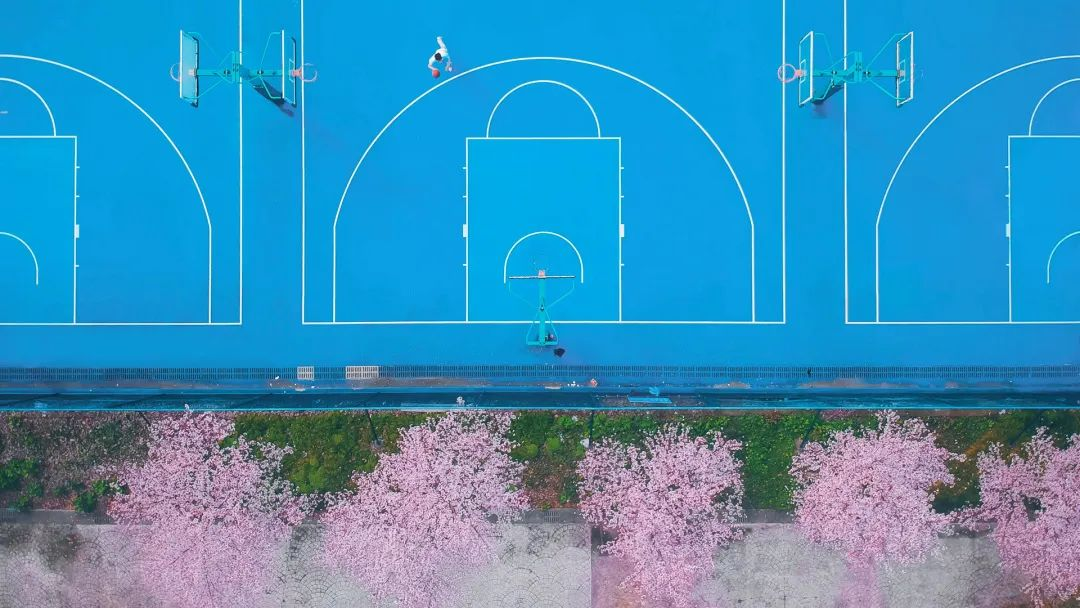
\includegraphics[width=0.3\textwidth]{./images/img3}
    \caption{原始图片}
\end{figure}

\begin{figure}[h]
    \centering
    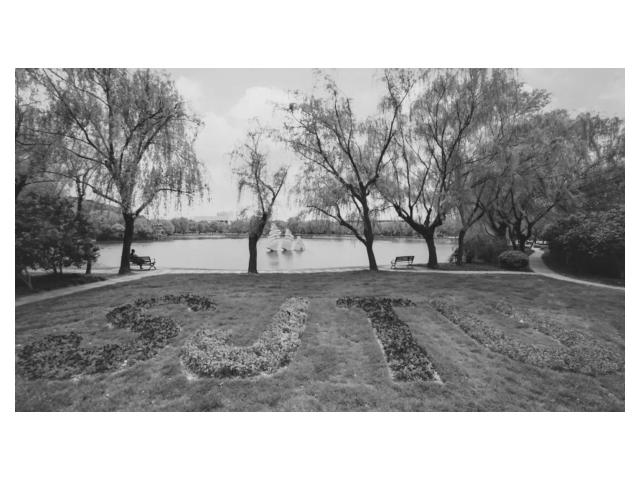
\includegraphics[width=0.3\textwidth]{./greyimages/img1}
    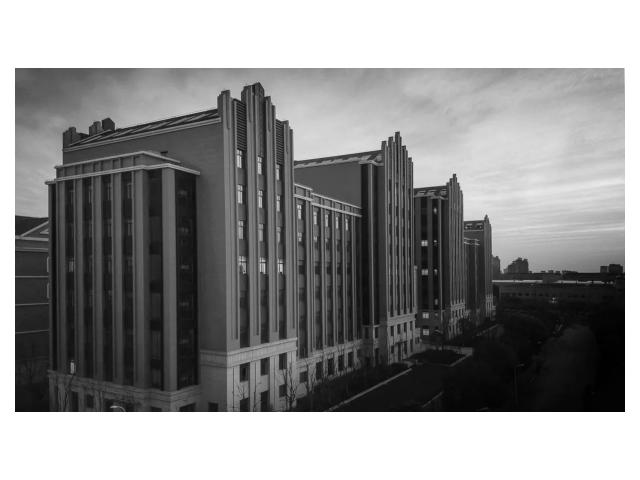
\includegraphics[width=0.3\textwidth]{./greyimages/img2}
    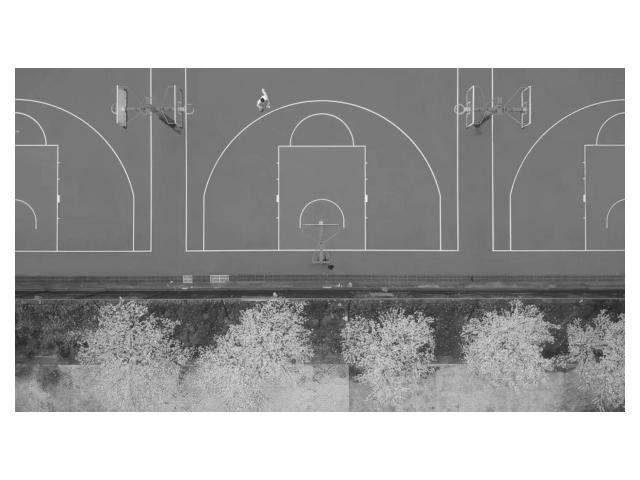
\includegraphics[width=0.3\textwidth]{./greyimages/img3}
    \caption{原始图片的灰度图}
\end{figure}

    第一张图片以绿植为主,绿色居多;第二张图片表现夕阳时的场景,红色居多;第三张图片主体是蓝色的球场,蓝色居多。
    这与颜色直方图表现的接近,说明颜色直方图能较好的表现图片的颜色特征。


    第一、二张图片的天空对应灰度图右侧的两个峰,第三张图片下方的部分对应灰度图中间的峰
    (即浅色部分)而第一张图片的草地,第二张图片的建筑物对应灰度图左侧的峰,第三章图片
    上方的部分对应灰度图的底部(即深色部分),灰度图基本反映了图片的亮暗特征。

    同时,第一张图片物体较多,变化大;第二张图次之,第三章图又次之,可以看到梯度强度图
    中,第一张图的梯度范围大,第二张图较小,第三张图几乎没有。梯度图反映了图片纹理的疏
    密程度,也可以反映高频特征和低频特征的分布情况。

\section{实验感想}
    第一次实验总体而言代码难度不大。借助实验,我学习了定量评估一个复杂的对象的方法,
    同时练习了python中绘图函数的使用,收获比较大。

    期间主要遇到了pyplot函数在使用中文作为图片标题时会导致乱码的问题,而后通过引入
    windows自带的微软雅黑字体避免了乱码的产生。

    同时,还尝试了批量处理图片的方法。尽管本次实验仅有三张图片,可以使用手动处理的方
    法,但批量处理对于后续实验的数据处理等很有帮助,不因数据量少就降低对自己的要求。
    
\end{document}
